\section{Experiments}
\label{sec:experiments}

\begin{figure}[t]
    % \vspace{-5pt}
    \centering
    % 去掉了 height=1\textwidth，让 LaTeX 自动保持原图比例
    \includegraphics[width=\textwidth]{Figures/step_compare.pdf}
    \caption{\textbf{Qualitative results in real-world and simulated manipulation tasks.} We evaluate on three challenging tasks: (a) Block Building, demanding precise bottom-to-top assembly toward a target configuration; (b) Block Disassembly, requiring structured top-to-bottom deconstruction and rearrangement; and (c) Block Hide and Restore, requiring causal memory maintenance under full occlusion. RoboStream consistently outperforms SoFar~\cite{qisofar} and VoxPoser~\cite{huang2023voxposer}, particularly in spatio-temporal perception and causal memory over extended horizons.}
    \label{fig:step_setting}
    % \vspace{-2em}

    % \centering
    % 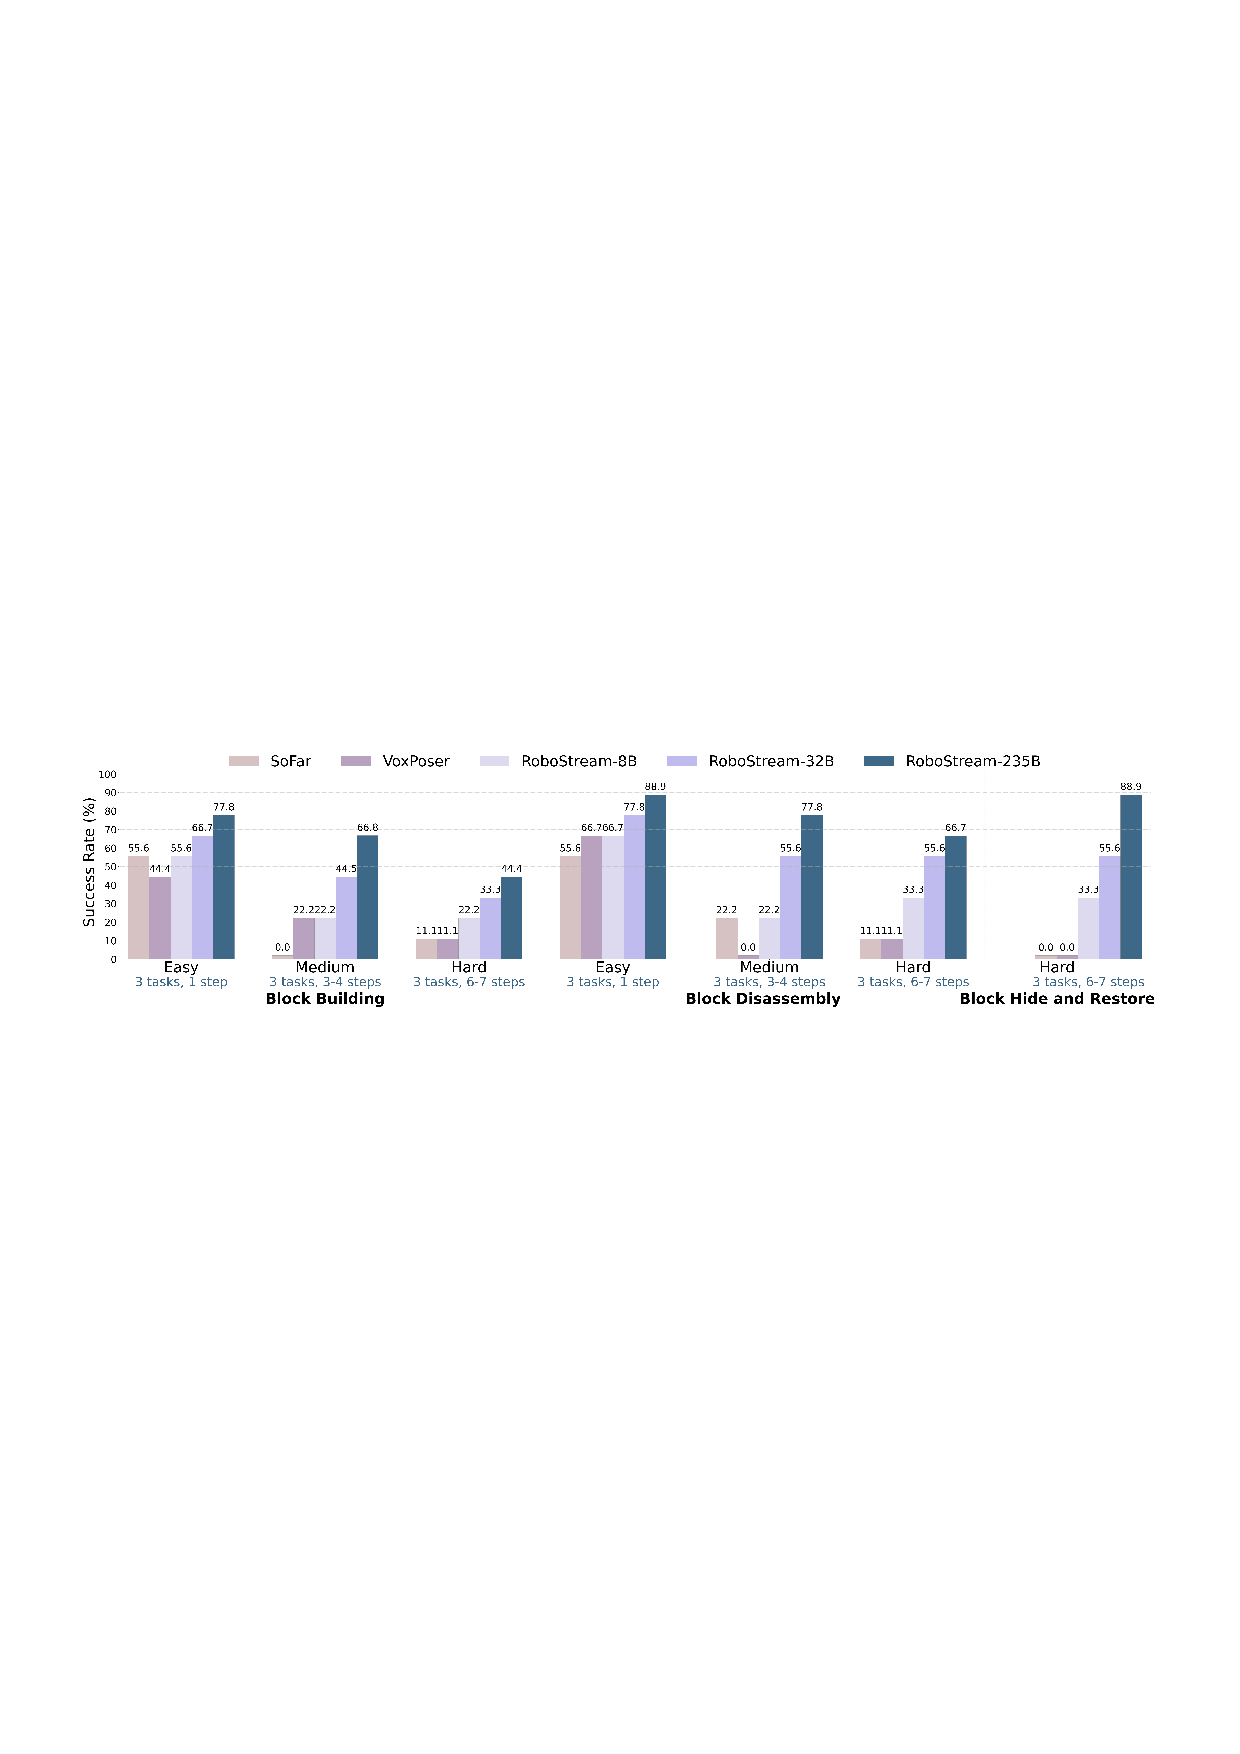
\includegraphics[width=1\textwidth]{Figures/1.pdf}
    % \caption{Performance comparison of RoboStream and baselines on real-world block building and disassembly across difficulty levels.}
    % \label{fig:real_world}
\end{figure}

\subsection{Experimental Setup}
\label{sec:setup}

We evaluate RoboStream across five benchmarks spanning physical and simulated environments, covering real-world manipulation on a Franka Research 3 arm (Sec.~\ref{sec:real_world}), long-horizon tasks on RLBench~\cite{james2020rlbench} (Sec.~\ref{sec:rlbench}), zero-shot generalization on SIMPLER~\cite{li2025evaluating} (Sec.~\ref{sec:simpler}), and 6-DoF spatial reasoning on SpatialBench~\cite{qisofar} and Open6DOR V2~\cite{ding2024open6dor} (Sec.~\ref{sec:spatial_reasoning}). short-horizon evaluation validates that the geometry grounding of STF-Tokens suppresses spatial hallucination in individual actions; long-horizon evaluation tests whether the full framework sustains causal state tracking and correct action ordering. We instantiate RoboStream with three VLM backbones, Qwen3-VL-8B, Qwen3-VL-32B, and Qwen3-VL-235B~\cite{yang2025qwen3}, hereafter referred to as RoboStream-8B, RoboStream-32B, and RoboS\-tream-235B respectively. All variants operate in a manner without environment-specific adaptation or fine-tuning across any benchmark. We compare against state-of-the-art baselines including SoFar~\cite{qisofar}, VoxPoser~\cite{huang2023voxposer}, and RT-2-X~\cite{zitkovich2023rt}, measuring execution success rate for manipulation tasks and accuracy for spatial reasoning.

To accommodate task diversity, we adopt two goal-specification strategies. For real-world experiments and RLBench long-horizon tasks, where target configurations are difficult to fully capture in text, we employ image-guided goal specification with images depicting the desired final state, such as blocks arranged in a target tower configuration. For SIMPLER short-horizon tasks, and tasks involving occlusion or state restoration, we employ text-guided natural language instructions, such as ``hide the blue cube, then restore the original state.''



\begin{figure}[t]
   
    \centering
    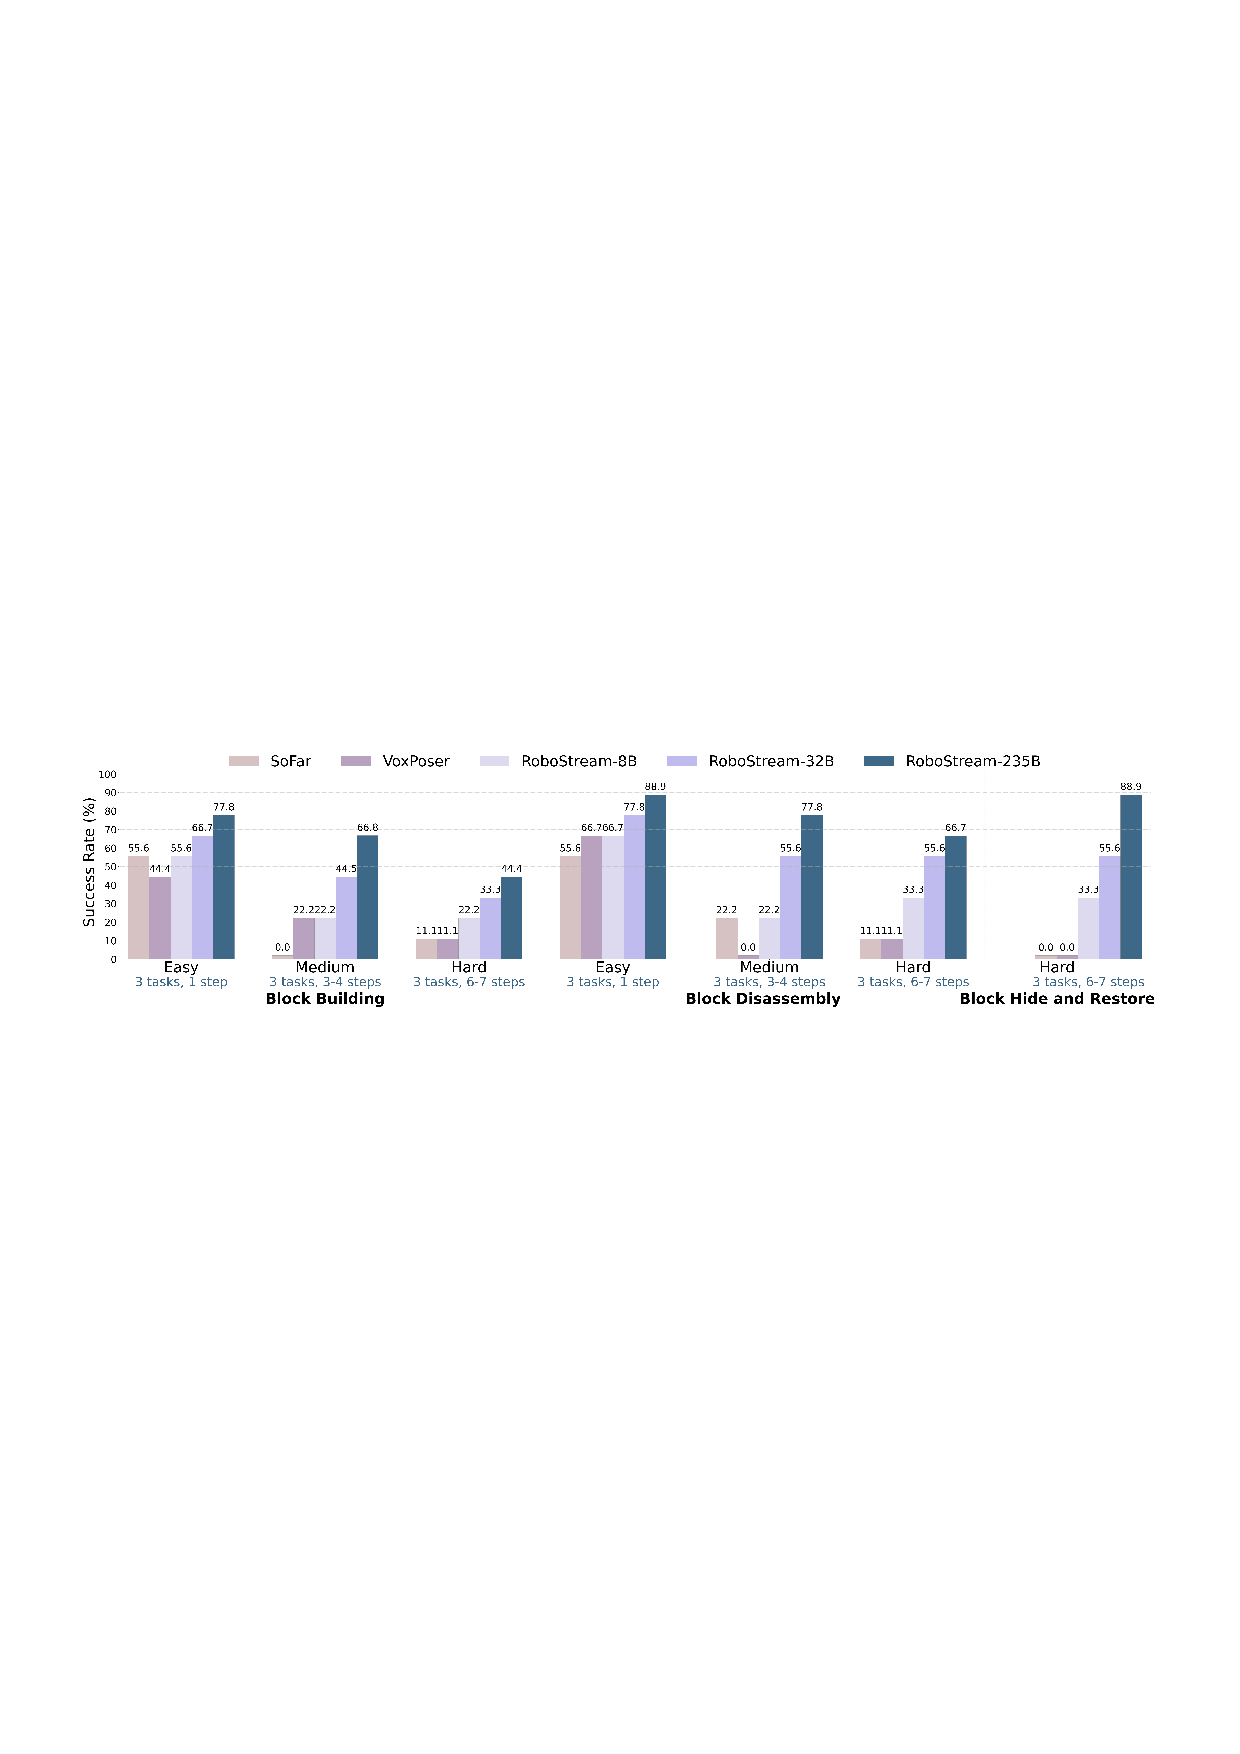
\includegraphics[width=1\textwidth]{Figures/1.pdf}
    \caption{\textbf{Performance comparison on zero-shot real-world manipulation tasks.} We design 21 diverse tasks covering block building (Task A), block disassembly (Task B), and block hide and restore (Task C).}
    \label{fig:real_world}
\end{figure}




\subsection{Real-World Robotic Manipulation}
\label{sec:real_world}
\noindent{\textbf{Tasks and Evaluations.}}~
We construct 21 real-world tasks on a Franka Research 3 (FR3) arm equipped with a parallel gripper and a front-view Intel RealSense D435i RGB-D camera, utilizing 17 colored objects, as shown in Fig.~\ref{fig:step_setting}. The tasks are categorized into three types evaluating different cognitive and physical reasoning dimensions. Task A (Block Building) assesses spatio-temporal grounding and pre-condition adherence by stacking objects Bottom-to-Top across three difficulty levels (Easy, Medium, Hard), requiring the robot to verify base stability before proceeding. Task B (Block Disassembly) evaluates sequential state tracking and support relation maintenance during Top-to-Bottom removal, requiring accurate causal memory of stacking order and support dependencies. Task C (Block Hide and Restore) stress-tests causal memory and object permanence under full occlusion, where the robot must conceal a block beneath a cup, execute distractor steps, and restore the original configuration by retrieving object identity and last known pose from causal history. Tasks A and B are specified by goal images, while Task C is guided by natural language instructions. Each task is executed three times, with details in the Appendix.




\noindent{\textbf{Results.}}~
As shown in Fig.~\ref{fig:real_world}, all RoboStream variants consistently outperform baselines across all difficulty levels, with success rates scaling proportionally with backbone capacity. On Hard-level block building and disassembly tasks, RoboStream-235B achieves success rates of 44.4\% and 66.7\%, respectively. In contrast, prior reactive systems such as SoFar~\cite{qisofar} and VoxPoser~\cite{huang2023voxposer} exhibit limited efficacy, struggling to exceed 11.1\% without persistent causal tracking and physical state evolution awareness. In Task C (Block Hide and Restore), requiring accurate tracking under total occlusion, RoboStream-235B achieves 88.9\% while even our lightweight 8B variant maintains 33.3\%, whereas SoFar and VoxPoser completely fail at 0\%. This contrast highlights that structured spatio-temporal memory is far more decisive for hidden-state tasks than scaling reactive systems. The monotonic gains across model scales confirm that STF-Tokens and CSTG provide complementary capabilities growing increasingly effective with model capacity, yielding robustness that purely reactive systems cannot replicate.

\begin{table*}[t]
    \centering
    \caption{\textbf{Quantitative success rate comparison on the SIMPLER benchmark}. We evaluate: (a) the Google Robot setup under Variant Aggregation (VA) and Visual Matching (VM) protocols, and (b) the WidowX + Bridge setup. For the WidowX tasks, we use the following abbreviations: Spoon (Put Spoon on Towel), Carrot (Put Carrot on Plate), Stack (Stack Green Block on Yellow Block), and Egg (Put Eggplant in Basket). ``Zero'' in the Data column indicates zero-shot evaluation. }
    \label{tab:simpler_env}

    % --- 左表 (Google Robot) ---
    \begin{minipage}[htbp]{0.42\linewidth}
        \centering
        \textbf{(a) Google Robot Setup}
        \vspace{2pt}

        \resizebox{\linewidth}{!}{%
        \renewcommand{\arraystretch}{1.1}
            \begin{tabular}{llcc}
                \toprule
                \textbf{Set} & \textbf{Policy} & \textbf{Pick Coke} & \textbf{Move Near} \\
                \midrule

                % --- VA 区块 ---
                \multirow{6}{*}{\textbf{VA}}
                & RT-1-X~\cite{brohan2022rt}     & 49.0 & 32.3 \\
                & RT-2-X~\cite{zitkovich2023rt}     & 82.3 & 79.2 \\
                & Octo-B~\cite{team2024octo}     & 0.6  & 3.1 \\
                & OpenVLA~\cite{kim2025openvla}    & 54.5 & 47.7 \\
                & SoFar~\cite{qisofar}      & \cellcolor{secondpurple}\underline{90.7} & \cellcolor{secondpurple}\underline{74.0} \\
                & \textbf{RoboStream-8B} & \cellcolor{firstpurple}\textbf{94.2} & \cellcolor{firstpurple}\textbf{79.8} \\
                \midrule

                % --- VM 区块 ---
                \multirow{6}{*}{\textbf{VM}}
                & RT-1-X~\cite{brohan2022rt}     & 56.7 & 31.7 \\
                & RT-2-X~\cite{zitkovich2023rt}     & 78.7 & 77.9 \\
                & Octo-B~\cite{team2024octo}     & 17.0 & 4.2 \\
                & OpenVLA~\cite{kim2025openvla}    & 16.3 & 46.2 \\
                & SoFar~\cite{qisofar}      & \cellcolor{secondpurple}\underline{92.3} & \cellcolor{secondpurple}\underline{91.7} \\
                & \textbf{RoboStream-8B} & \cellcolor{firstpurple}\textbf{95.7} & \cellcolor{firstpurple}\textbf{95.8} \\
                \bottomrule
            \end{tabular}
        }
    \end{minipage}
    \hfill
    % --- 右表 (WidowX) ---
    \begin{minipage}[htbp]{0.56\linewidth}
        \centering
        \textbf{(b) WidowX + Bridge Setup}
        \vspace{2pt}

        \renewcommand{\arraystretch}{1.11}
        \resizebox{\linewidth}{!}{%
            \begin{tabular}{llccccc}
                \toprule
                \textbf{Policy} & \textbf{Data} & \textbf{Spoon} & \textbf{Carrot} & \textbf{Stack} & \textbf{Egg} & \textbf{Avg} \\
                \midrule
                RT-1-X~\cite{brohan2022rt}      & OXE    & 0.0 & 4.2 & 0.0 & 0.0 & 1.1 \\
                Octo-B~\cite{team2024octo}      & OXE    & 12.5 & 8.3 & 0.0 & 43.1 & 16.0 \\
                Octo-S~\cite{team2024octo}      & OXE    & 47.2 & 9.7 & 4.2 & 56.9 & 30.0 \\
                OpenVLA~\cite{kim2025openvla}    & OXE    & 0.0 & 0.0 & 0.0 & 4.1 & 1.0 \\
                RoboVLM~\cite{li2026robovlm}     & OXE    & 20.8 & 25.0 & 8.3 & 0.0 & 13.5 \\
                RoboVLM~\cite{li2026robovlm}     & Bridge & 29.2 & 25.0 & 12.5 & 58.3 & 31.3 \\
                SpatialVLA~\cite{qu2025spatialvla}  & OXE    & 20.8 & 20.8 & 25.0 & 70.8 & 34.4 \\
                SpatialVLA~\cite{qu2025spatialvla}  & Bridge & 16.7 & 25.0 & 29.2 & \cellcolor{firstpurple}\textbf{100.0} & 42.7 \\
                SoFar~\cite{qisofar}       & Zero   & \cellcolor{secondpurple}\underline{58.3} & \cellcolor{secondpurple}\underline{66.7} & \cellcolor{secondpurple}\underline{70.8} & 37.5 & \cellcolor{secondpurple}\underline{58.3} \\
                \midrule
                \textbf{RoboStream-8B} & \textbf{Zero} & \cellcolor{firstpurple}\textbf{62.5} & \cellcolor{firstpurple}\textbf{71.9} & \cellcolor{firstpurple}\textbf{77.1} & \cellcolor{secondpurple}\underline{87.5} & \cellcolor{firstpurple}\textbf{74.8} \\
                \bottomrule
            \end{tabular}
        }
    \end{minipage}
\end{table*}

\subsection{Simulation Object Manipulation Evaluation on SIMPLER}
\label{sec:simpler}

We evaluate zero-shot cross-embodiment generalization on the SIMPLER benchmark~\cite{li2025evaluating} across Google Robot and WidowX + Bridge configurations, representing substantial domain shifts from training environments. These short-horizon tasks isolate STF-Token contributions by testing whether spatial grounding transfers across embodiments and viewpoints, independent of long-horizon reasoning.

\noindent{\textbf{Google Robot Configuration.}}~
As shown in Tab.~\ref{tab:simpler_env}, RoboStream-8B achieves superior success rates on both ``Pick Coke Can'' and the spatially demanding ``Move Near'' tasks under VM evaluation, surpassing the prior state-of-the-art SoFar~\cite{qisofar}. Notably, RoboStream-8B also outperforms OXE-finetuned RT-2-X~\cite{zitkovich2023rt} by a substantial margin despite operating fully zero-shot. Under the more challenging VA evaluation, RoboStream-8B maintains competitive performance, again exceeding SoFar. Consistent gains across both protocols and tasks with varying geometry confirm stable spatial grounding independent of embodiment.

\noindent{\textbf{WidowX + Bridge Configuration.}}~
RoboStream achieves a higher average success rate across all subtasks compared to zero-shot SoFar and Bridge-finetuned SpatialVLA~\cite{qu2025spatialvla} without requiring any fine-tuning or domain adaptation. Notably, this advantage holds despite SpatialVLA being explicitly trained on in-domain Bridge data, highlighting the superior transferability of our geometry-grounded representation. These results confirm that spatio-temporal reasoning grounded in explicit geometric primitives transfers robustly across embodiments and extends naturally from short tasks to subsequent long-horizon benchmarks.





\subsection{Simulation Long-Horizon Task Evaluation on RLBench}
\label{sec:rlbench}


\begin{table}[t]
\centering
\caption{\textbf{Simulation evaluation of long-horizon manipulation on RLBench.} All RoboStream variants are evaluated in a zero-shot manner without in-domain fine-tuning. }
\label{tab:full_vertical_compact}
\resizebox{\textwidth}{!}{
\begin{tabular}{l ccccc}
\toprule
\textbf{Tasks} & 
\textbf{SoFar}~\cite{qisofar} & 
\textbf{VoxPoser}~\cite{huang2023voxposer} & 
\textbf{RoboStream-8B} & 
\textbf{RoboStream-32B} & 
\textbf{RoboStream-235B} \\
\midrule
Bridge Between Towers            & 52.0 & 8.0 & \cellcolor{secondpurple}\underline{76.0} & \cellcolor{firstpurple}\textbf{88.0} & \cellcolor{firstpurple}\textbf{88.0} \\
Cover Top Block with Box         & 4.0 & 4.0 & 40.0 & \cellcolor{secondpurple}\underline{84.0} & \cellcolor{firstpurple}\textbf{92.0} \\
Cover Bottom Block with Box      & 0.0 & 0.0 & 16.0 & \cellcolor{secondpurple}\underline{68.0} & \cellcolor{firstpurple}\textbf{96.0} \\
Place Blocks in Two Containers   & \cellcolor{firstpurple}\textbf{100.0} & \cellcolor{secondpurple}\underline{96.0} & \cellcolor{firstpurple}\textbf{100.0} & \cellcolor{firstpurple}\textbf{100.0} & \cellcolor{firstpurple}\textbf{100.0} \\
Place Blocks in Two Cont. (Hard) & 4.0 & 4.0 & 24.0 & \cellcolor{secondpurple}\underline{76.0} & \cellcolor{firstpurple}\textbf{88.0} \\
Stack Five Colors                & 4.0 & 4.0 & 60.0 & \cellcolor{secondpurple}\underline{72.0} & \cellcolor{firstpurple}\textbf{80.0} \\
Stack Three Colors               & \cellcolor{secondpurple}\underline{60.0} & \cellcolor{firstpurple}\textbf{96.0} & \cellcolor{firstpurple}\textbf{96.0} & \cellcolor{firstpurple}\textbf{96.0} & \cellcolor{firstpurple}\textbf{96.0} \\
Unstack then Stack Four Colors   & 0.0 & 0.0 & 52.0 & \cellcolor{secondpurple}\underline{76.0} & \cellcolor{firstpurple}\textbf{84.0} \\
\midrule
\textbf{Average}                     & 28.0 & 26.5 & 58.0 & \cellcolor{secondpurple}\underline{82.5} & \cellcolor{firstpurple}\textbf{90.5} \\
\bottomrule
\end{tabular}
}
\end{table}

\noindent{\textbf{Tasks and Evaluations.}}~
To assess long-horizon manipulation capabilities, we introduce 8 complex tasks within RLBench~\cite{james2020rlbench} (Tab.~\ref{tab:full_vertical_compact}), constructed by extending and reconfiguring native assets. Each method is evaluated over 25 episodes per task using different random seeds. Following Sec.~\ref{sec:setup}, tasks are categorized by guidance modality. Five goal-image-guided tasks require visually complex target configurations, including Bridge Between Towers, Place Blocks in Two Containers, Place Blocks in Two Cont. (Hard), and Stack Three/Five Colors. Three text-guided tasks stress-test action ordering, restoration, and object permanence under occlusion, including Cover Top/Bottom Block with Box and Unstack then Stack Four Colors. Detailed setups are provided in the Appendix.

\noindent{\textbf{Results.}}~
As shown in Tab.~\ref{tab:full_vertical_compact}, RoboStream consistently outperforms both SoFar~\cite{qisofar} and VoxPoser~\cite{huang2023voxposer} across these long-horizon scenarios. Notably, our framework demonstrates a strong scaling effect, with performance increasing alongside model capacity to reach a 90.5\% average success rate on RoboStream-235B without additional training, as larger capacity provides the reasoning depth necessary to maintain logical consistency over extended action sequences. However, scaling the VLM alone is not a panacea for long-horizon stability. Even our smallest variant, RoboStream-8B, substantially exceeds much larger baselines, demonstrating that spatio-temporal reasoning and structured memory are more critical for physical consistency than simply increasing parameter scale.










\begin{table}[t]
    \centering
    % --- 左侧表格 ---
    \begin{minipage}[t]{0.56\textwidth} 
        \centering
        \vspace{0em}
        \setlength{\tabcolsep}{2.5pt} 
        \caption{\textbf{Spatial reasoning evaluation on 6-DoF SpatialBench~\cite{qisofar}.} Results are categorized by spatial VQA task types, covering absolute ($abs.$) and relative ($rel.$) reasoning for both position and orientation.}
        \label{tab:spatial_reasoning_final}
        \scriptsize
        \begin{tabular}{@{}lccccc@{}}
        \toprule
        \multirow{2}{*}{Method} & \multicolumn{2}{c}{Position} & \multicolumn{2}{c}{Orientation} & \multirow{2}{*}{Total} \\
        \cmidrule(lr){2-3} \cmidrule(lr){4-5}
        & rel. & abs. & rel. & abs. & \\
        \midrule
        GPT-4o~\cite{hurst2024gpt}      & 49.4 & 28.4 & 44.2 & 25.8 & 36.2 \\
        SpaceMantis~\cite{chen2024spatialvlm} & 33.6 & 29.2 & 27.2 & 25.0 & 28.9 \\
        RoboPoint~\cite{yuan2025robopoint}   & 43.8 & 30.8 & 33.8 & 25.8 & 33.5 \\
        SoFar~\cite{qisofar} & 59.6 & 33.8 & \cellcolor{firstpurple}\textbf{54.6} & 31.3 & 43.9 \\
        SoFar-8B~\cite{qisofar} & 41.5 & 24.3 & 27.1 & 31.3 & 30.5 \\
        SoFar-32B~\cite{qisofar} & \cellcolor{secondpurple}\underline{60.4} & \cellcolor{secondpurple}\underline{41.9} & 45.8 & 33.3 & \cellcolor{secondpurple}\underline{45.3} \\
        \textbf{RoboStream-8B} & 47.2 & 31.1 & 35.4 & \cellcolor{secondpurple}\underline{35.4} & 36.8 \\
        \textbf{RoboStream-32B} & \cellcolor{firstpurple}\textbf{66.0} & \cellcolor{firstpurple}\textbf{44.6} & \cellcolor{secondpurple}\underline{48.0} & \cellcolor{firstpurple}\textbf{37.5} & \cellcolor{firstpurple}\textbf{48.9} \\
        \bottomrule
        \end{tabular}
    \end{minipage}
    \hfill 
    % --- 右侧表格 ---
    \begin{minipage}[t]{0.42\textwidth} % 保持宽度 0.42
        \centering
        \setlength{\tabcolsep}{2pt} % 保持 2pt
        \renewcommand{\arraystretch}{1.18} % 
        \caption{\textbf{6-DoF object rea\-r\-r\-a\-n\-g\-e\-m\-e\-n\-t evaluation on O\-p\-e\-n\-6\-D\-O\-R~\cite{ding2024open6dor}.} Results are categorized by position ($Pos.$), rotation ($Rot.$), and integrated 6-DoF success rates. }
        \label{tab:open6dor_updated}
        \scriptsize 
        \begin{tabular}{@{}lccc@{}}
        \toprule
        Method & Pos.  & Rot.  & 6-DoF  \\
        \midrule
        Dream2Real~\cite{kapelyukh2024dream2real}         & 15.9 & 31.3 & 13.5 \\
        VoxPoser~\cite{huang2023voxposer}            & 32.6 & -    & -    \\
        Open6DOR-GPT~\cite{ding2024open6dor}       & 74.9 & 41.1 & 35.6 \\
        SoFar~\cite{qisofar}          & 93.0 & \cellcolor{secondpurple}\underline{57.0} & \cellcolor{secondpurple}\underline{48.7} \\
        SoFar-8B~\cite{qisofar}               & 92.4 & 42.9 & 45.1 \\
        SoFar-32B~\cite{qisofar}              & \cellcolor{secondpurple}\underline{93.1} & 54.6 & 48.4 \\
        \textbf{RoboStream-8B}          & \cellcolor{secondpurple}\underline{93.1} & 47.6 & 47.3 \\
        \textbf{RoboStream-32B}& \cellcolor{firstpurple}\textbf{93.8} & \cellcolor{firstpurple}\textbf{58.8} & \cellcolor{firstpurple}\textbf{52.2} \\
        \bottomrule
        \end{tabular}
    \end{minipage}
\end{table}



\subsection{6-DoF Spatial Reasoning Evaluation}
\label{sec:spatial_reasoning}
To evaluate how STF-Tokens bridge high-level visual features with precise instance-level 3D grounding, we extend our evaluation to rotation and full 6-DoF pose estimation. Following SoFar~\cite{qisofar}, we incorporate PointSO for 6-DoF prediction and evaluate on Open6DOR V2~\cite{ding2024open6dor} and 6-DoF SpatialBench~\cite{qisofar}. Since SoFar serves as our primary baseline, we include variants using Qwen3-VL-8B and Qwen3-VL-32B backbones for fair cross-scale comparison with RoboStream.



\noindent{\textbf{Spatial Reasoning on 6-DoF SpatialBench.}}~
As shown in Tab.~\ref{tab:spatial_reasoning_final}, RoboStream-32B achieves superior overall performance, outperforming both SoFar and GPT-4o~\cite{hurst2024gpt}. The most pronounced gains appear on absolute and relative position tasks, where pure image-text alignment is most susceptible to spatial ambiguity. These results confirm that the core advantage of STF-Tokens lies not in coordinate injection alone, but in serving as a geometric anchor providing deterministic spatial reference when visual features and language descriptions conflict.



\noindent{\textbf{6-DoF Object Rearrangement on Open6DOR V2.}}~
As shown in Tab.~\ref{tab:open6dor_updated}, RoboStream-32B consistently outperforms SoFar across position, rotation, and integrated 6-DoF metrics. Unlike baselines treating spatial coordinates as text annotations, STF-Tokens distill per-object visual evidence into structured instance representations encoding centroid, Gaussian shape, and orientation. This shift from pixel-level to object-level reasoning underlies consistent gains across all tracks, most notably on 6-DoF where tight placement constraints demand precise geometric grounding and spatial alignment.

\begin{table*}[t]
\centering
\caption{\textbf{Ablation study on RoboStream-235B.} Success rates (\%) across 8 long-horizon tasks, isolating contributions of CSTG and STF-Tokens.}
\label{tab:ablation_235b_horizontal}
\resizebox{\textwidth}{!}{%
\renewcommand{\arraystretch}{1.2} % 稍微增加行高，让色块更美观
\begin{tabular}{cc | ccccccccc}
\toprule
\thead{\textit{STF-} \\ \textit{Tokens}} & \thead{\textit{CSTG}} &
 \thead{Bridge Between\\Towers} & 
 \thead{Cover Top\\Block} & 
 \thead{Cover Bottom\\Block} & 
 \thead{Place in\\Containers} & 
 \thead{Place in\\Containers (Hard)} & 
 \thead{Stack Five\\Colors} & 
 \thead{Stack Three\\Colors} & 
 \thead{Unstack then\\Stack} & 
 \textbf{Average} \\
\midrule
% w/o Both (Baseline)
\xmark & \xmark & 0.0 & 0.0 & 0.0 & 84.0 & 12.0 & 0.0 & 0.0 & 0.0 & 12.0 \\
% w/o CSTG
\cmark & \xmark & 0.0 & 0.0 & 0.0 & \cellcolor{secondpurple}\underline{92.0} & 24.0 & 0.0 & 0.0 & 0.0 & 14.5 \\
% w/o STF-Tokens
\xmark & \cmark & \cellcolor{secondpurple}\underline{72.0} & \cellcolor{secondpurple}\underline{84.0} & \cellcolor{secondpurple}\underline{88.0} & \cellcolor{firstpurple}\textbf{100.0} & \cellcolor{secondpurple}\underline{72.0} & \cellcolor{secondpurple}\underline{60.0} & \cellcolor{firstpurple}\textbf{96.0} & \cellcolor{secondpurple}\underline{64.0} & \cellcolor{secondpurple}\underline{79.5} \\
% Full Model
\cmark & \cmark & \cellcolor{firstpurple}\textbf{88.0} & \cellcolor{firstpurple}\textbf{92.0} & \cellcolor{firstpurple}\textbf{96.0} & \cellcolor{firstpurple}\textbf{100.0} & \cellcolor{firstpurple}\textbf{88.0} & \cellcolor{firstpurple}\textbf{80.0} & \cellcolor{firstpurple}\textbf{96.0} & \cellcolor{firstpurple}\textbf{84.0} & \cellcolor{firstpurple}\textbf{90.5} \\
\bottomrule
\end{tabular}%
}
\end{table*}



\subsection{Ablation Study}
\label{sec:ablation_study}

We ablate RoboStream-235B across all 8 long-horizon RLBench~\cite{james2020rlbench} tasks to isolate the contribution of each architectural component (Tab.~\ref{tab:ablation_235b_horizontal}). Removing the CSTG module (\textit{w/o CSTG}) causes the average success rate to collapse from 90.5\% to 14.5\%, confirming that persistent state tracking is the foundational driver for long-horizon tasks. However, while CSTG provides logical structure, STF-Tokens provide physical precision. Removing STF-Tokens (\textit{w/o STF-Tokens}) results in an 11.0\% absolute drop (from 90.5\% to 79.5\%), demonstrating that without explicit 3D geometric grounding, even a CSTG-equipped agent struggles with compounding spatial inaccuracies during contact-rich execution. The mutual dependence of both components becomes evident when removing them simultaneously (\textit{w/o Both}), which yields only 12.0\% success rate. Notably, comparing this to the \textit{w/o CSTG} variant (14.5\%) shows that STF-Tokens still provide marginal improvement in short-horizon spatial accuracy even when long-horizon logic fails. Their full potential, however, is unlocked only when coupled with the CSTG, where CSTG ensures correct action sequencing and STF-Tokens ensure each step is executed with deterministic spatial precision.

% %3.5 12:29 wujie修改
% We ablate RoboStream-235B across eight long-horizon RLBench tasks to isolate the contribution of each architectural component (Tab.~\ref{tab:ablation_235b_horizontal}). Removing the causal memory log (\textit{w/o Memory}) leads to a catastrophic performance collapse, confirming that persistent state tracking is the foundational driver for long-horizon tasks. While memory provides logical structure, STF-Tokens offer essential physical precision. Eliminating STF-Tokens (\textit{w/o STF-Tokens}) results in a significant performance drop, demonstrating that without explicit 3D geometric grounding, even a memory-equipped agent struggles with compounding spatial inaccuracies during contact-rich execution. The mutual dependence of both components becomes evident in the \textit{w/o Both} variant, which fails to complete nearly all tasks. Notably, comparing this to the \textit{w/o Memory} baseline suggests that STF-Tokens still provide marginal improvements in local spatial accuracy even when long-horizon logic fails. Their full potential, however, is unlocked only when coupled with the causal memory log: memory ensures correct action sequencing, while STF-Tokens guarantee that each step is executed with deterministic spatial precision.